Les figures~2 et~3 comparent les huit stratégies évaluées : les stratégies de référence issues des travaux précédents (\texttt{Standard\_First}, \texttt{Standard\_Rkt}, \texttt{LFT2\_Energy}) et nos stratégies développées cette année (\texttt{APE\_H\_Hybrid}, \texttt{RL\_PPO}, \texttt{Meta\_Agent}, \texttt{DQN}). Les expériences ont été conduites sur une machine de 16 cœurs et 16\,Go de RAM.

\begin{figure}[htbp]
    \centering
    \begin{minipage}[b]{0.49\textwidth}
        \centering
        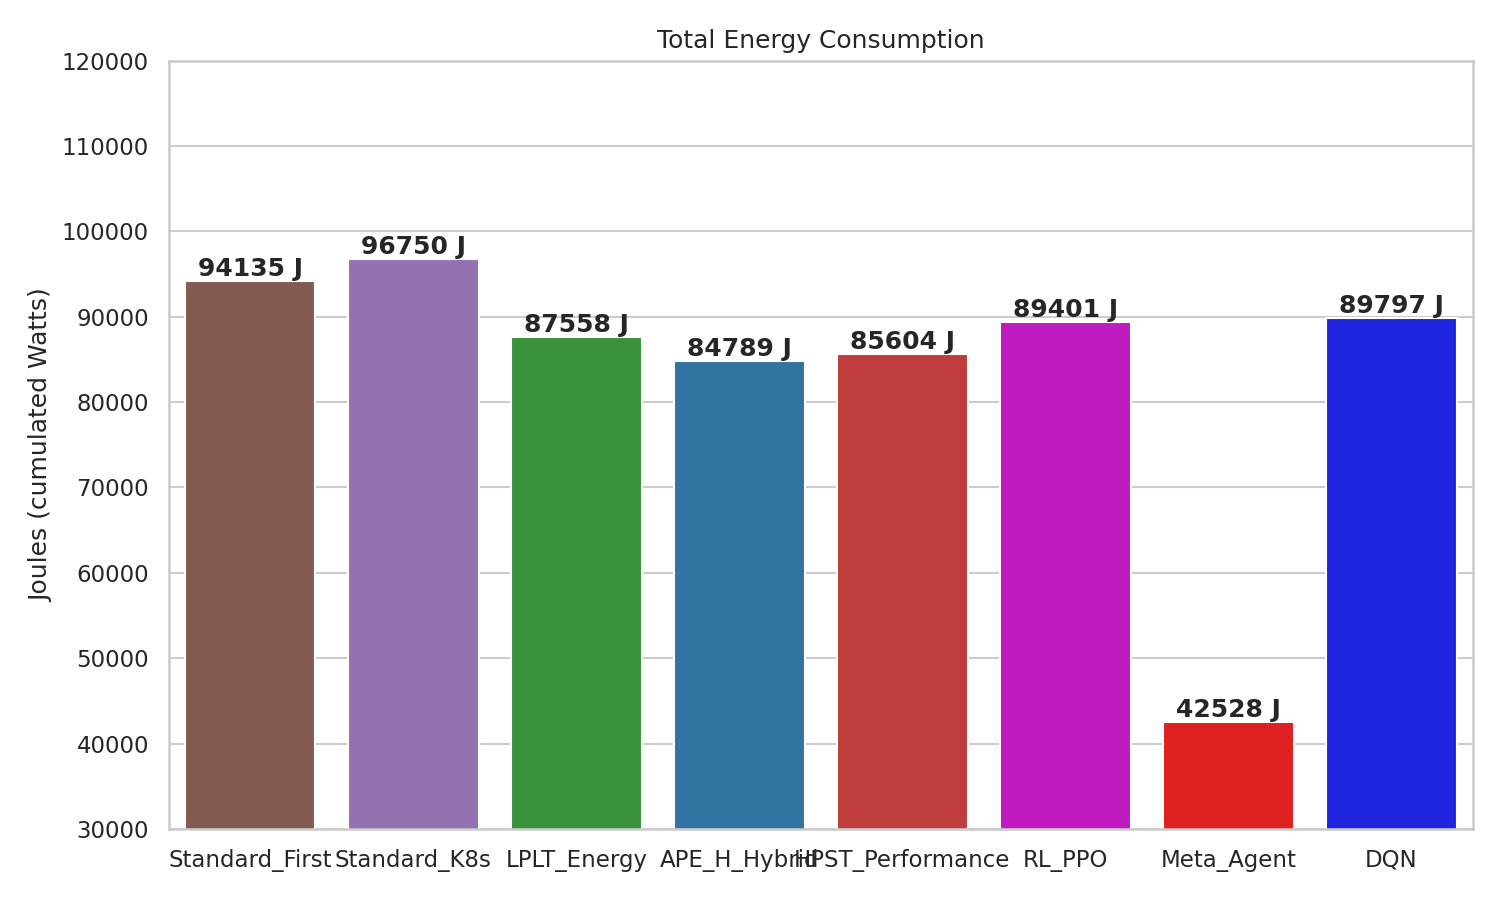
\includegraphics[width=\textwidth]{images/plot_energy.png}
        \caption{Comparaison de la consommation énergétique totale des stratégies}
        \label{fig:energy}
    \end{minipage}
    \hfill
    \begin{minipage}[b]{0.49\textwidth}
        \centering
        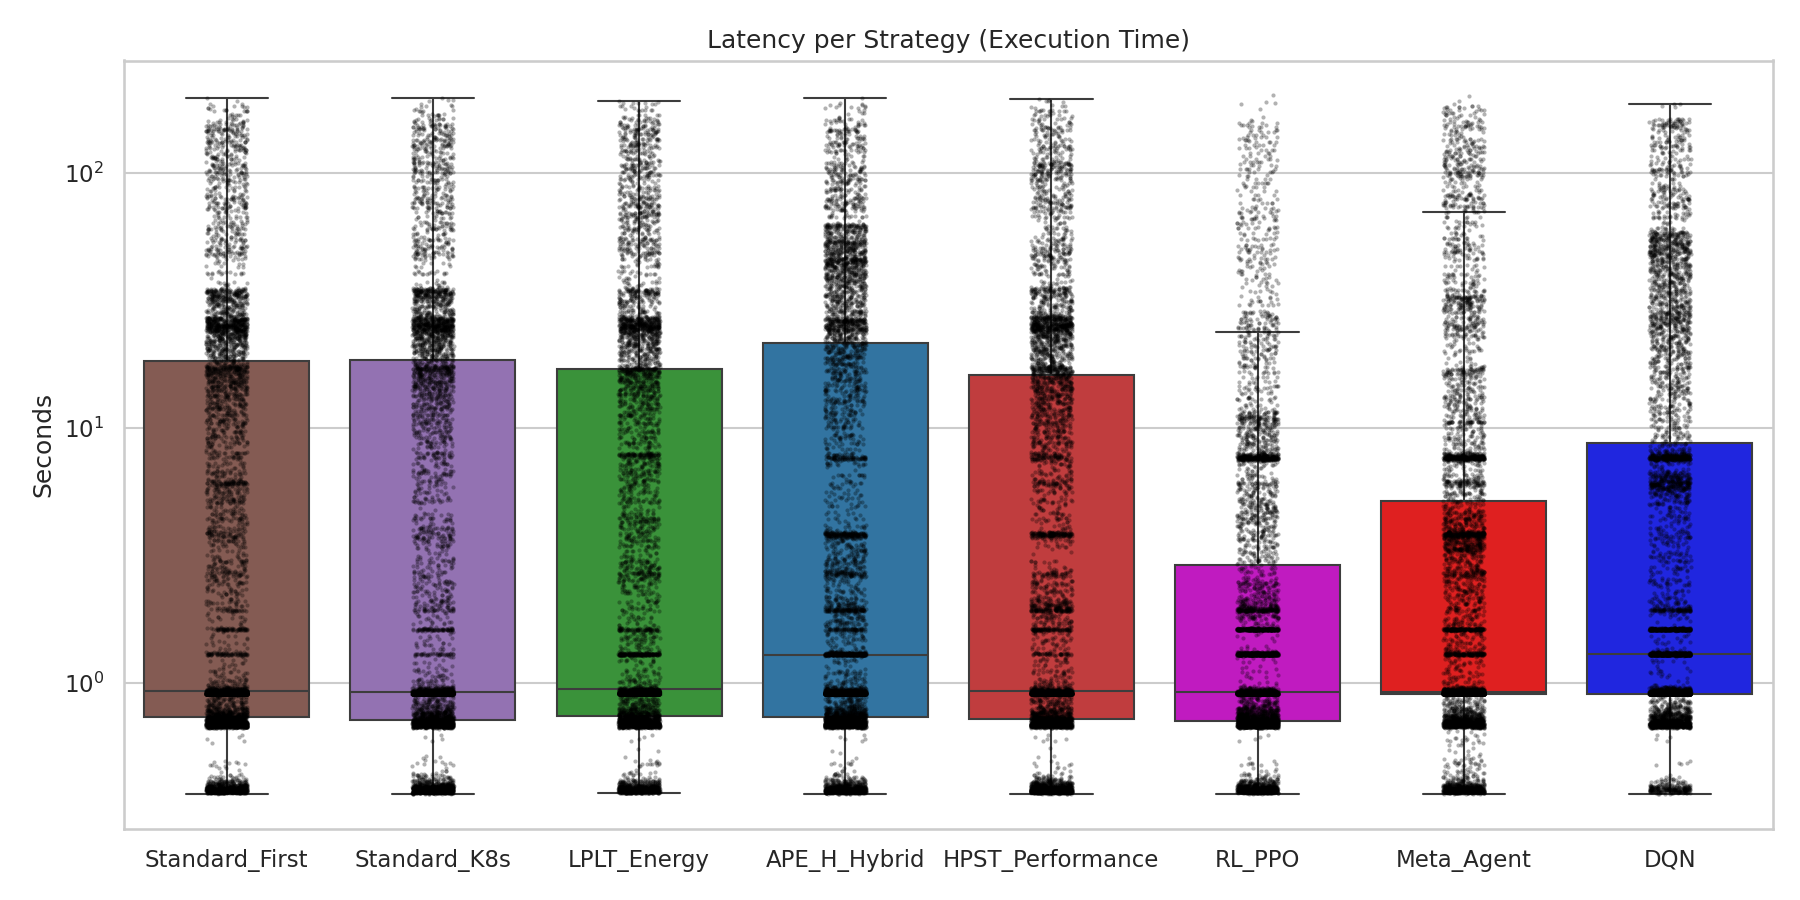
\includegraphics[width=\textwidth]{images/plot_latency.png}
        \caption{Boxplot de la distribution de la latence pour chaque stratégie}
        \label{fig:latency}
    \end{minipage}
\end{figure}

Côté économie énergétique, l'approche décentralisée (\texttt{Meta\_Agent}) et l'algorithme hybride (\texttt{APE\_H\_Hybrid}) sont les plus économes, loin devant les méthodes classiques. En revanche, sur la latence, l'agent \texttt{RL\_PPO} est de loin le plus performant : il est le seul à traiter presque toutes les requêtes en moins d'une seconde. En résumé, le \texttt{PPO} offre le meilleur équilibre global entre économie énergétique et temps de réponse.
